%----------------------------------------------------------------------------------------
%	PACKAGES AND OTHER DOCUMENT CONFIGURATIONS
%----------------------------------------------------------------------------------------

\documentclass[11pt, notitlepage]{article} % Default font size and suppress title page

\usepackage[utf8]{inputenc} % Required for inputting international characters
\usepackage[T1]{fontenc} % Output font encoding for international characters
% A note on fonts: As of 2019, NIH allows Arial, Georgia, Helvetica, and Palatino Linotype. Georgia and Arial are commercial fonts so you will need to use XeLaTeX and have them installed on your machine to use them. Palatino & Helvetica are available as free LaTeX packages so select the one you want and comment out the other.
\usepackage{palatino} % Palatino font
\linespread{1.05} % A little extra line spread is better for the Palatino font
%\usepackage{helvet} % Helvetica font
\renewcommand*\familydefault{\sfdefault} % Use the sans serif version of the font

\usepackage{amsfonts, amsmath, amsthm, amssymb} % For math fonts, symbols and environments
\usepackage{graphicx} % Required for including images
\usepackage{booktabs} % Nice rules in tables
\usepackage{wrapfig} % Required for text to wrap around figures and tables
\usepackage[labelfont=bf]{caption} % Make figure numbering in captions bold
\usepackage[top=0.5in,bottom=0.5in,left=0.5in,right=0.5in]{geometry} % Page margins
\pagestyle{empty} % Suppress headers and footers

\hyphenation{ionto-pho-re-tic iso-tro-pic fortran} % Specifies custom hyphenation points for words or words that shouldn't be hyphenated at all

%----------------------------------------------------------------------------------------

\begin{document}

%----------------------------------------------------------------------------------------
%	GENERAL INFORMATION
%----------------------------------------------------------------------------------------

\begin{center}
{\Large \textbf{Project Description:}\\  
\vspace{.5cm}
{\LARGE\textbf{Project Name}} 
\\[.75cm] 
submitted by\\
{Yernur Baibolatov\\
Universit\"at Potsdam\\
Institut f\"ur Physik und Astronomie}
\end{center}
%\\[.75cm] 
\noindent\textbf{Specific academic field (specialization)}: Planetology?
\\[.75cm] 
\textbf{Supervisor and first expert reviewer for recommendation letters}: Prof. Dr. Frank Spahn
\\[.75cm] 
\textbf{Further expert reviewers (name, academic field; these do not have to be identical with the second reviewer of the PhD thesis)}: ???
\\[.75cm] 
\textbf{Working environment}: Please  briefly  explain  how you  are  integrated  in  colloquia, a  working  group,   a  research  training group etc.  Please indicate if you are an individual doctoral student.

\section*{Abstract}
Clear  and  comprehensible  presentation  of  the  project,  short  characterization  of  your  project’s  objectives (not longer than 15 lines)


%----------------------------------------------------------------------------------------
%	Summary of the research topic
%----------------------------------------------------------------------------------------

\newpage

\section*{A. Summary of the research topic}

\begin{description} % For subheadings within a section, this template uses the {description} environment, it is not obtrusively large like a \subsection; and facilitates a brief optional subtitle; and it will wrap around figures and tables; it also has a decent amount of whitespace above/below which is less than for a section heading
	\item[A.1. Instructions.]{Optional subtitle}
\end{description}

Explain the importance of the problem or critical barrier to progress in the field that the proposed project addresses.

Explain how the proposed project will improve scientific knowledge, technical capability, and/or clinical practice in one or more broad fields.

Describe how the concepts, methods, technologies, treatments, services, or preventative interventions that drive this field will be changed if the proposed aims are achieved.

\begin{description}
	\item[A.2. Subheading.]{}
\end{description}

\begin{wraptable}{l}{5.5cm} % Example table with text wrapping around it
	\caption{Example Table}
	\begin{center}
		\begin{tabular}{l l r}
			\toprule
			\multicolumn{1}{c}{City} & {N\textsuperscript{a}} & {\%Silly}\\
			\midrule
			San Diego & 289 & 41\%\\
			Seattle & 262 & 32\%\\
			Galveston & 261 & 15\%\\
			St Louis & 269 & 7\%\\
			New York & 271 & 4\%\\
			Baltimore & 231 & 2\%\\
			\emph{Total} & 1,586 & 21\%\\
			\hline 
		\end{tabular}\\
		\footnotesize\textsuperscript{a}{All participants clowns.}
	\end{center}
	\label{tab:example}
\end{wraptable}

Referencing a table using it's label: Table \ref{tab:example}. Maecenas consectetur metus at tellus finibus condimentum. Proin arcu lectus, ultrices non tincidunt et, tincidunt ut quam. Integer luctus posuere est, non maximus ante dignissim quis. Nunc a cursus erat. Curabitur suscipit nibh in tincidunt sagittis. Nam malesuada vestibulum quam id gravida. Proin ut dapibus velit. Vestibulum eget quam quis ipsum semper convallis. Duis consectetur nibh ac diam dignissim, id condimentum enim dictum. Nam aliquet ligula eu magna pellentesque, nec sagittis leo lobortis. Aenean tincidunt dignissim egestas. Morbi efficitur risus ante, id tincidunt odio pulvinar vitae. Proin ut dapibus velit. Vestibulum eget quam quis ipsum semper convallis. Duis consectetur nibh ac diam dignissim, id condimentum enim dictum.

Curabitur tempus hendrerit nulla. Donec faucibus lobortis nibh pharetra sagittis. Sed magna sem, posuere eget sem vitae, finibus consequat libero. Cras aliquet sagittis erat ut semper. Aenean vel enim ipsum. Fusce ut felis at eros sagittis bibendum mollis lobortis libero. Donec laoreet nisl vel risus lacinia elementum non nec lacus. Nullam luctus, nulla volutpat ultricies ultrices, quam massa placerat augue, ut fringilla urna lectus nec nibh. Vestibulum efficitur condimentum orci a semper. Pellentesque ut metus pretium lacus maximus semper. Sed tellus augue, consectetur rhoncus eleifend vel, imperdiet nec turpis. Nulla ligula ante, malesuada quis orci a, ultricies blandit elit.

In malesuada ullamcorper urna, sed dapibus diam sollicitudin non. Donec elit odio, accumsan ac nisl a, tempor imperdiet eros. Donec porta tortor eu risus consequat, a pharetra tortor tristique. Morbi sit amet laoreet erat. Morbi et luctus diam, quis porta ipsum. Quisque libero dolor, suscipit id facilisis eget, sodales volutpat dolor. Nullam vulputate interdum aliquam. Mauris id convallis erat, ut vehicula neque. Sed auctor nibh et elit fringilla, nec ultricies dui sollicitudin.

\begin{wrapfigure}{r}{8.5cm} % Example figure with text wrapping around it
	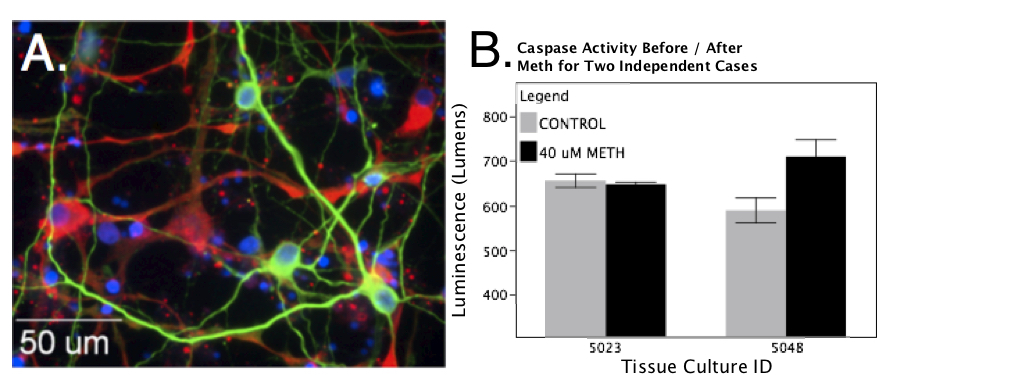
\includegraphics[width=8.2cm]{Figures/Fig1.jpg}
	\caption{\footnotesize Example wrapped figure. (A) Impressive microscopy image. (B) Impressive data.}
	\label{fig:example}
\end{wrapfigure}

Referencing a figure using it's label: Figure \ref{fig:example}. Proin lobortis efficitur dictum. Pellentesque vitae pharetra eros, quis dignissim magna. Sed tellus leo, semper non vestibulum vel, tincidunt eu mi. Aenean pretium ut velit sed facilisis. Ut placerat urna facilisis dolor suscipit vehicula. Ut ut auctor nunc. Nulla non massa eros. Proin rhoncus arcu odio, eu lobortis metus sollicitudin eu. Duis maximus ex dui, id bibendum diam dignissim id. Aliquam quis lorem lorem. Phasellus sagittis aliquet dolor, vulputate cursus dolor convallis vel. Suspendisse eu tellus feugiat, bibendum lectus quis, fermentum nunc. Nunc euismod condimentum magna nec bibendum. Curabitur elementum nibh eu sem cursus, eu aliquam leo rutrum. Sed bibendum augue sit amet pharetra ullamcorper. Aenean congue sit amet tortor vitae feugiat. Vestibulum vestibulum luctus metus venenatis facilisis. Suspendisse iaculis augue at vehicula ornare. Sed vel eros ut velit fermentum porttitor sed sed massa. Fusce venenatis, metus a rutrum sagittis, enim ex maximus velit, id semper nisi velit eu purus.

\begin{description}
	\item[A.3. Another subheading:]{optional subtitle.}
\end{description}

In congue risus leo, in gravida enim viverra id. Donec eros mauris, bibendum vel dui at, tempor commodo augue. In vel lobortis lacus. Nam ornare ullamcorper mauris vel molestie. Maecenas vehicula ornare turpis, vitae fringilla orci consectetur vel. Nam pulvinar justo nec neque egestas tristique. Donec ac dolor at libero congue varius sed vitae lectus. Donec et tristique nulla, sit amet scelerisque orci. Maecenas a vestibulum lectus, vitae gravida nulla. Proin eget volutpat orci. Morbi eu aliquet turpis. Vivamus molestie urna quis tempor tristique. Proin hendrerit sem nec tempor sollicitudin.

\begin{figure}[b] % Figure at bottom of the page ([b] argument, could be "t" for top or "h" for here)
	\centering
	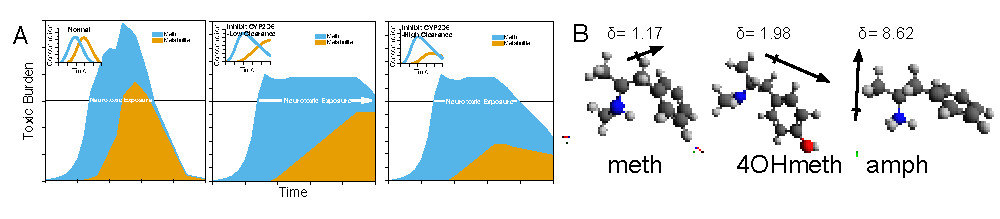
\includegraphics[scale = .80]{Figures/Fig2.pdf}
	\caption{\footnotesize Big Figure legend Big Figure legend Big Figure legend Big Figure legend Big Figure legend Big Figure legend Big Figure legend Big Figure legend Big Figure legend.}
	\label{fig2}
\end{figure}

Fusce eleifend porttitor arcu, id accumsan elit pharetra eget. Mauris luctus velit sit amet est sodales rhoncus. Donec cursus suscipit justo, sed tristique ipsum fermentum nec. Ut tortor ex, ullamcorper varius congue in, efficitur a tellus. Vivamus ut rutrum nisi. Phasellus sit amet enim efficitur, aliquam nulla id, lacinia mauris. Quisque viverra libero ac magna maximus efficitur. Interdum et malesuada fames ac ante ipsum primis in faucibus. Vestibulum mollis eros in tellus fermentum, vitae tristique justo finibus. Sed quis vehicula nibh. Etiam nulla justo, pellentesque id sapien at, semper aliquam arcu. Integer at commodo arcu. Quisque dapibus ut lacus eget vulputate.

Vestibulum sodales orci a nisi interdum tristique. In dictum vehicula dui, eget bibendum purus elementum eu. Pellentesque lobortis mattis mauris, non feugiat dolor vulputate a. Cras porttitor dapibus lacus at pulvinar. Praesent eu nunc et libero porttitor malesuada tempus quis massa. Aenean cursus ipsum a velit ultricies sagittis. Sed non leo ullamcorper, suscipit massa ut, pulvinar erat. Aliquam erat volutpat. Nulla non lacus vitae mi placerat tincidunt et ac diam. Aliquam tincidunt augue sem, ut vestibulum est volutpat eget. Suspendisse potenti. Integer condimentum, risus nec maximus elementum, lacus purus porta arcu, at ultrices diam nisl eget urna. Curabitur sollicitudin diam quis sollicitudin varius. Ut porta erat ornare laoreet euismod. In tincidunt purus dui, nec egestas dui convallis non. In vestibulum ipsum in dictum scelerisque.

\begin{description}
	\item[A.4. Yet another subheading.]{}
\end{description}

Aenean feugiat pellentesque venenatis. Sed faucibus tristique tortor vel ultrices. Donec consequat tellus sapien. Nam bibendum urna mauris, eget sagittis justo gravida vel. Mauris nisi lacus, malesuada sit amet neque ut, venenatis tempor orci. Curabitur feugiat sagittis molestie. Duis euismod arcu vitae quam scelerisque facilisis. Praesent volutpat eleifend tortor, in malesuada dui egestas id. Donec finibus ac risus sed pellentesque. Donec malesuada non magna nec feugiat. Mauris eget nibh nec orci congue porttitor vitae eu erat. Sed commodo ipsum ipsum, in elementum neque gravida euismod. Cras mi lacus, pulvinar ut sapien ut, rutrum sagittis dui. Donec non est a metus varius finibus. Pellentesque rutrum pellentesque ligula, vitae accumsan nulla hendrerit ut.

In mi mauris, finibus non faucibus non, imperdiet nec leo. In erat arcu, tincidunt nec aliquam et, volutpat eget nisl. Vivamus id eros scelerisque est condimentum condimentum at at ligula. Proin blandit sapien ac bibendum faucibus. Nunc sem elit, blandit in lectus vitae, lacinia hendrerit risus. Donec efficitur elementum massa, eget interdum nunc porttitor sed. Aenean porttitor gravida nibh, vel bibendum tellus. Nunc fermentum lobortis nunc. Cras aliquet odio mauris, eget lobortis metus lacinia sit amet. Maecenas id elit eu orci ornare ultricies. Sed consequat turpis id accumsan malesuada. Fusce varius imperdiet ex, vel sodales purus scelerisque id. Morbi ut tellus interdum, laoreet leo non, dignissim odio. Nunc vel quam diam. Sed eu tortor in dolor mattis rhoncus.

%----------------------------------------------------------------------------------------
%	Table of contents and outline of the thesis with an overview of accomplished (sub-) chapter
%----------------------------------------------------------------------------------------

\newpage
\section*{B.Table of contents and outline of the thesis with an overview of accomplished (sub-) chapter}
Please submit your table of contents /outline of your thesis. Please characterize the (sub-)chapter that have already been accomplished. The probability of concluding the project during the funding period  must  be  illustrated.  The awarding committee reserves the right to obtain the stated (sub-) chapter in printed form.

%----------------------------------------------------------------------------------------
%	Working program and intended completion date
%----------------------------------------------------------------------------------------

\newpage
\section*{C. Working program and intended completion date}
\begin{itemize}
    \item Working-Program, time schedule (max. 4 pages)Detailed information about your planned approach, especially a thorough explanation of the meth-odology, that you will apply in the completion phase of your  PhD. A time schedule (e. g. in graphic or  tabular  form)  for  the  period  of  funding  should  clearly  demonstrate  the  steps  in  your  research  project that are planned, have already started or are completed. If your PhD includes experiments, please indicate the experiments that have already been conducted and that will still be conducted. The  quality  of  the  research  approach  and  the  characterization  of  the  accomplished  and  planned  steps are of utmost importance.
    \item Please specify your intended completion date.
\end{itemize}
%----------------------------------------------------------------------------------------
%	Literature
%----------------------------------------------------------------------------------------

\newpage
\section*{D. Literature}

\newpage

\bibliography{NIHGrant} % Use the NIHGrant.bib file for the reference list, replace with your own
\bibliographystyle{nihunsrt} % Use the custom nihunsrt bibliography style included with the template

%----------------------------------------------------------------------------------------

\end{document}